\chapter{Sequential Backdoor 
Adjustment Formula}
\label{ch-seq-bdoor}

\begin{figure}[h!]
\centering
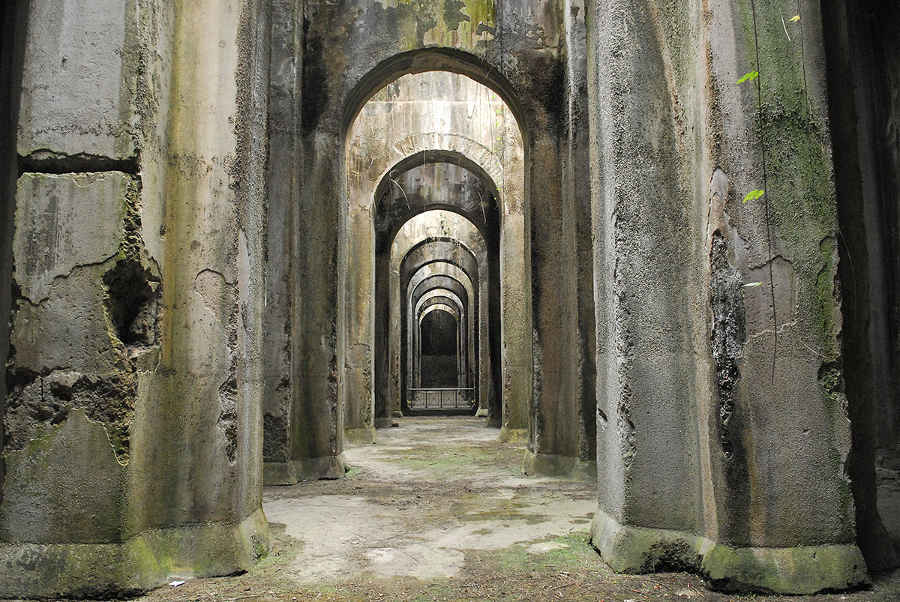
\includegraphics[width=5in]
{piscina-mirabilis.jpeg}
\caption{Piscina Mirabilis, 
ancient Roman cistern in Naples} 
\label{fig-piscina}
\end{figure}


This chapter is based
on Ref.\cite{pearl-robins-95}
by Pearl and Robins.

The goal of this
chapter is to 
generalize 
the backdoor adjustment
formula (see Chapter \ref{ch-bdoor})
from 
a query $P(y|\cald\rvx=x)$
with a single
do node to a query 
$P(y|\cald\rvx^n=x^n)$
with multiple
do nodes. 


For $n=1,2,3 \ldots$, define 
\beqa
\calq(y|x^n)&=&
\sum_{z^n}
P(y|x^n, z^n)
\prod_{t=0}^{n-1}
P(z_t|x_{<t}, z_{<t})
\\
&&
\xymatrix{
&\sum_{z^n}
\\
=
}
\xymatrix{
z^n\ar[d]
\\
y
\\
x^n\ar[u]
}
\xymatrix{\\
\prod_{t=0}^{n-1}}
\xymatrix{
z_{<t}\ar[r]
&z_t
\\
\\
x_{<t}\ar[uur]
}
\label{def-q-y-xn-seqbdoor}
\eeqa

For $n=1$,
\beq
\xymatrix{\\
\calq(y|x_0)
}
\xymatrix{
&\sum_{z_0}
\\
=
}
\xymatrix{
z_0\ar[d]
\\
y
\\
x_0\ar[u]
}
\xymatrix{P(z_0)\\ \\}
\xymatrix{
\\
=\quad
}
\xymatrix{
\sum z_0\ar[dr]
\\
& y
\\
x_0\ar[ur]
}
\;.
\eeq

For $n=2$, 

\begin{align}
\xymatrix{
\\
\calq(y|x^2)
}
&
\xymatrix{
&\sum_{z^2}
\\
=
}
\xymatrix{
(z_0,z_1)\ar[d]
\\
y
\\
(x_0,x_1)\ar[u]
}
\xymatrix{
P(z_0)
}
\xymatrix{
z_0\ar[r]
&z_1
\\
\\
x_0\ar[ruu]
}
\\
&
\xymatrix{\\=}
\xymatrix{
\sum z_0\ar[r]\ar[drr]
&\sum z_1\ar[dr]
\\
&&y
\\
x_0\ar[ruu]\ar[urr]
&x_1\ar[ur]
}
\;.
\end{align}

For $n=3$, 

\begin{align}
\xymatrix{\\
\calq(y|x^3)
}
&
\xymatrix{
&\sum_{z^3}
\\
=
}
\xymatrix{
(z_0,z_1,z_2)\ar[d]
\\
y
\\
(x_0,x_1, x_2)\ar[u]
}
\xymatrix{
P(z_0)
}
\xymatrix{
z_0\ar[r]
&z_1
\\
\\
x_0\ar[ruu]
}
\xymatrix{
(z_0,z_1)\ar[r]
&z_2
\\
\\
(x_0,x_1)\ar[ruu]
}
\\
\nonumber
\\
&
\xymatrix{
&\sum_{z^3}
\\
=
}
\xymatrix{
(z_0,z_1,z_2)\ar[d]
\\
y
\\
(x_0,x_1, x_2)\ar[u]
}
\xymatrix{
P(z_0)
}
\xymatrix{
z_0\ar[r]\ar@/^1pc/[rr]
&z_1\ar[r]
&z_2
\\
\\
x_0\ar[uur]\ar[uurr]
&x_1\ar[uur]
&x_2
}
\\
\nonumber
\\
&
\xymatrix{\\=}
\xymatrix{
\sum z_0\ar[r]\ar@/^1pc/[rr]
\ar[drrr]
&\sum z_1\ar[r]
\ar[drr]
&\sum z_2
\ar[dr]
\\
&&&y
\\
x_0\ar[uur]\ar[uurr]
\ar[urrr]
&x_1\ar[uur]
\ar[urr]
&x_2
\ar[ur]
}
\end{align}



\SeqBdoorDef

\begin{claim}(Sequential 
Backdoor Adjustment Formula)

\SeqBdoorClaim
\end{claim}
\proof
If
$z^n$
satisfies the
backdoor
criterion
relative
to
$(\rvx^n, \rvy)$,
then
$\rvx^n, \rvy, \rvz^n$
might
have the following 
structure for $n=3$.

\beq
\xymatrix{
\rvz_0\ar[r]\ar@/^1pc/[rr]\ar[drrr]
\ar[dd]
&\rvz_1\ar[r]\ar[drr]
\ar[dd]
&\rvz_2\ar[dr]
\ar[dd]
\\
&&&\rvy
\\
\rvx_0\ar[uur]\ar[uurr]\ar[urrr]
\ar[r]\ar@/_1pc/[rr]
&\rvx_1\ar[uur]
\ar[urr]\ar[r]
&\rvx_2
\ar[ur]
}
\label{eq-bnet-bdoor-proof}
\eeq

One can check
using the following 3 
auxilliary bnets
that bnet Eq.(\ref{eq-bnet-bdoor-proof})
satisfies the
sequential backdoor
adjustment 
criterion.
Note that conditioned
nodes are shaded yellow.
\beq
\begin{array}{ccc}
\xymatrix@C=.95pc{
*++[o][F*:yellow]{\rvz_0}\ar[r]\ar@/^1pc/[rr]\ar[drrr]
\ar[dd]
&*++[o][F*:yellow]{\rvz_1}\ar[r]\ar[drr]
&*++[o][F*:yellow]{\rvz_2}\ar[dr]
\\
&&&\rvy
\\
\rvx_0
&\rvx_1\ar[uur]
\ar[urr]
&\rvx_2
\ar[ur]
}
&
\xymatrix@C=.95pc{
\rvz_0\ar[r]\ar@/^1pc/[rr]\ar[drrr]
\ar[dd]
&*++[o][F*:yellow]{\rvz_1}\ar[r]\ar[drr]
\ar[dd]
&*++[o][F*:yellow]{\rvz_2}\ar[dr]
\\
&&&\rvy
\\
*++[o][F*:yellow]{\rvx_0}
\ar[uur]\ar[uurr]\ar[urrr]\ar[r]
&\rvx_1
&\rvx_2
\ar[ur]
}
&
\xymatrix@C=.95pc{
\rvz_0\ar[r]\ar@/^1pc/[rr]\ar[drrr]
\ar[dd]
&\rvz_1\ar[r]\ar[drr]
\ar[dd]
&*++[o][F*:yellow]{\rvz_2}\ar[dr]
\ar[dd]
\\
&&&\rvy
\\
*++[o][F*:yellow]{\rvx_0}
\ar[uur]\ar[uurr]\ar[urrr]
\ar[r]\ar@/_1pc/[rr]
&*++[o][F*:yellow]{\rvx_1}\ar[uur]
\ar[urr]\ar[r]
&\rvx_2
}
\\
\\
\call_{\rvx_0}\cald_{\rvx_1, \rvx_2}G
&\call_{\rvx_1}\cald_{\rvx_2}G
&\call_{\rvx_2}G
\end{array}
\eeq



See Claim \ref{cl-decSeqBackDoor}
for a proof of this claim.
\qed



